\documentclass[a4paper]{article}
\usepackage{graphicx}
\usepackage{float}

\title{ISO/IEEE 11073-10206 - ACOM (Abstract Content Information Model)}
\author{Riccardo Cambianica}
\begin{document}
    \maketitle
    \tableofcontents
    \newpage
    
    \section{Ambito e finalità}
        Questo standard definisce un modello di contenuto astratto (ACOM: Abstract Content Information Model) per i dispositivi di salute personale. 
        L'obiettivo di IEEE 11073-10206 è quello di documentare le informazioni in un PHD e il contenuto delle osservazioni sanitarie che vengono inviati dal
        PHD in modo che quando un'osservazione viene ricevuta dal PHD, indipendentemente dal protocollo utilizzato per eseguire
        la comunicazione, le informazioni sanitarie sono \textbf{complete}, \textbf{coerenti} e \textbf{inequivocabili}.
        IEEE 11073-10206 definisce un modello informativo astratto ed object-oriented allo scopo di rappresentare un PHD (Personal Health Device) e le osservazioni che può generare.
        Specifica quali informazioni devono essere presenti e le relazioni tra elementi informativi nel modello. Modella le osservazioni in modo generico
        concentrandosi sulle informazioni contenuto nella presentazione delle misure sanitarie.
    
    \section{Contesto}
        La figura~\ref{fig:overallContextOfWork} mostra le categorie e i tipi tipici di dispositivi nell'ambito della salute personale. Dispositivi di salute personale, o PHD 
        (ad esempio: monitor della pressione sanguigna, bilance e pedometri) raccolgono informazioni su una o più persone, trasferendole poi ad un gateway
        di salute personale, o PHG (ad esempio: telefono cellulare, apparecchio sanitario o personal computer) per la raccolta, la visualizzazione 
        e l'eventuale trasmissione successiva. Il PHG può anche trasmettere i dati a servizi di supporto remoto per ulteriori analisi o per permettere la gestione delle malattie.
    \begin{figure}[H]
        \centering
        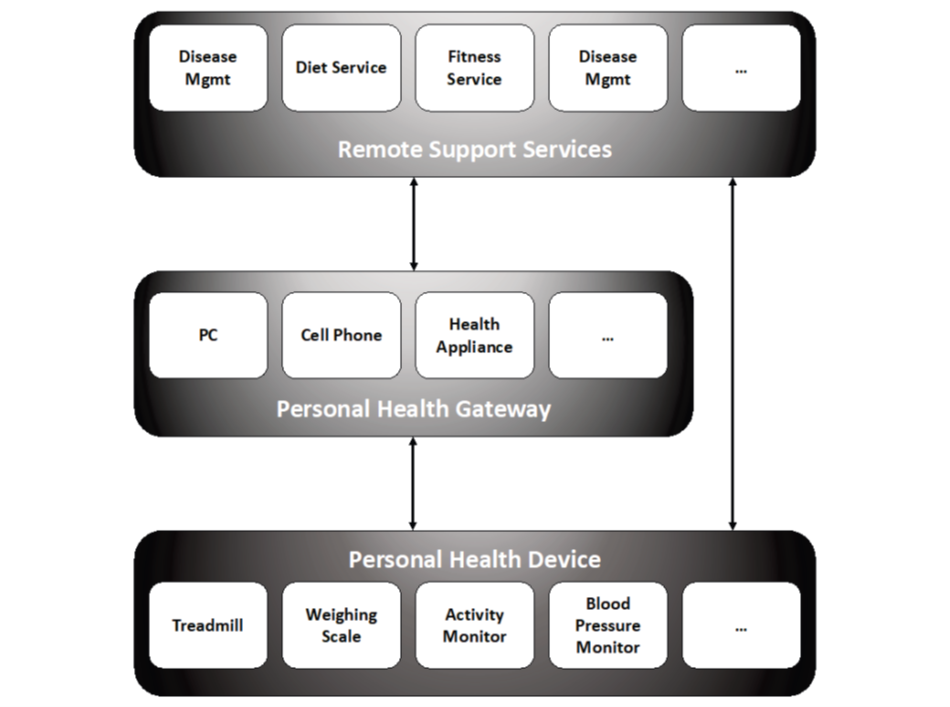
\includegraphics[width=1\textwidth]{figures/overall context of work.png}
        \caption{Overall context of work}
        \label{fig:overallContextOfWork}
    \end{figure}
    
    \section{ACOM Observation class}
    La classe di osservazione ACOM fornisce un modello generico per esprimere osservazioni da dispositivi di salute personale.
    E' basata sull'oggetto metrico descritto dallo standard ISO/IEEE 11073-20601 e condivide molti attributi della risorsa analoga osservazione presente nello standard HL7 FHIR.
    Come si può vedere in figura \ref{fig:observationClass}, la classe si compone di una serie di elementi concettuali, tutti derivanti dall'oggetto \textbf{Observation}.  
    \begin{figure}[H]
        \centering
        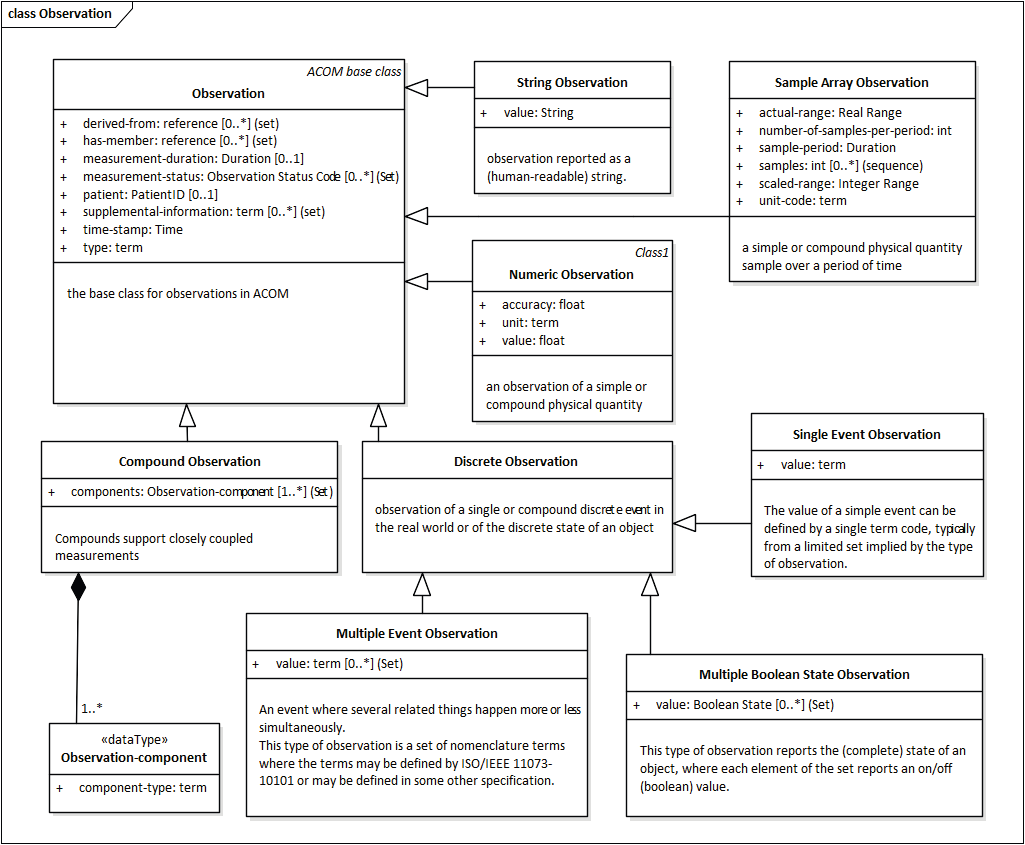
\includegraphics[width=1\textwidth]{figures/observation class.png}
        \caption{Classe Observation}
        \label{fig:observationClass}
    \end{figure}
    
\section{ACOM device specializations}
    Le specializzazioni dei dispositivi sono usate in questo standard per definire il contenuto informativo di uno specifico tipo di PHD.
    In parole povere sono classi che modellano alcuni tipi di PHD particolari (appartenenti alla classe IEEE 11073-104XX), di conseguenza contengono al loro interno le informazioni basiche sulla struttura del PHD (Power, Clock e SystemInfo), 
    un oggetto che modella il PHD e un oggetto Observation che modella le osservazioni. 
    Dato che il capitolo 8 del PDF su ACOM tratta tutti i tipi di PHD, userò il primo (un termometro), come esempio per gli altri.
    \newpage
    \subsection{IEEE 11073-10408 thermometer}
    \begin{figure}[H]
        \centering
        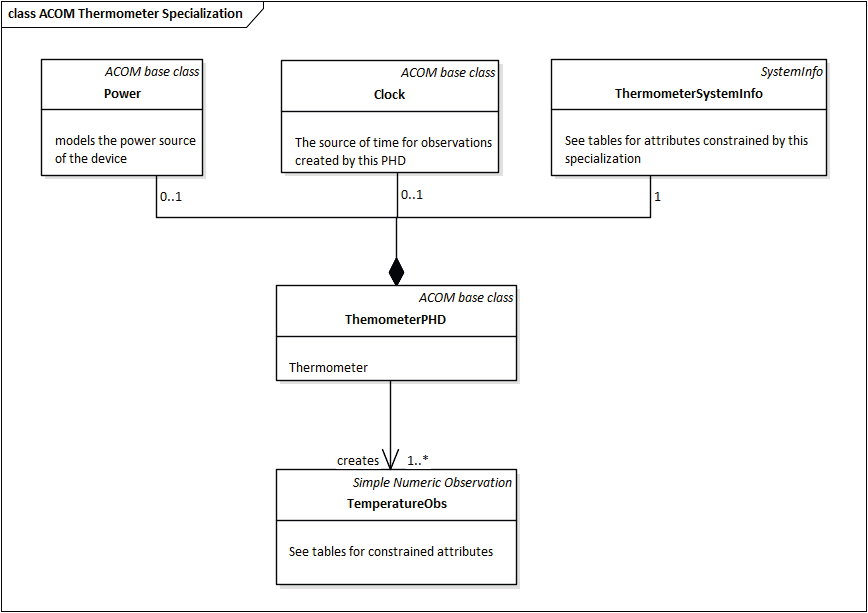
\includegraphics[width=1\textwidth]{figures/ACOM thermometer specialization class.png}
        \caption{class ACOM Thermometer Specialization}
    \end{figure}
\end{document}